\section{Dedicated Detectors for LLPs}
\subsection{Introduction}

Some boilerplate about how, in cases of ultra-low-mass particles, ultra-long lifetimes, or unusual LLP charged, it is hard to trigger on and/or reconstruct the events in the main ATLAS, CMS, and LHCb detectors. This has led to new proposals and experiments to look for LLPs in new regimes that are otherwise inaccessible at the LHC. These experiments provide the best sensitivity to new millicharged LLPs, magnetic monopoles, and other models such as Higgs-portal hidden sectors, dark photons, and Majorana neutrinos.


\subsection{A Compact Detector for Exotics at LHCb (CODEX-b)}
\label{sec:CODEX-b}

As discussed elsewhere in the white paper, LLPs are theoretically well motivated and come in wide range of masses and lifetimes. ATLAS and CMS have excellent sensitivity for fairly high mass LLP's, regardless of their lifetime  (see e.g.~\cite{CMS:2016ybj,Aaboud:2016dgf,CMS-PAS-EXO-16-003,ATLAS-CONF-2016-103}). Low mass and/or softer final states are more challenging due to both background and triggering limitations. In the short lifetime regime, for $c\tau$ of the scale of the VELO, LHCb has sensitivity to somewhat lower masses and can trigger on softer muonic final states, generating complementary reach provided the LLP has a significant branching ratio to muons~\cite{Aaij:2017mic,Aaij:2016xmb,Aaij:2016isa,Aaij:2015ica,Aaij:2014nma}. Finally the low mass/soft final states with rather long lifetimes are challenging for all three experiments. These signatures can be covered partially by NA62~\cite{NA62:2017rwk} operating in beam dump mode, or by SHiP~\cite{Alekhin:2015byh}, or by dedicated LHC experiments like MATHUSLA~\cite{Chou:2016lxi}, FASER~\cite{Feng:2017uoz} or CODEX-b \cite{Gligorov:2017nwh}. Of these options, only MATHUSLA and CODEX-b could gather a large sample Higgs bosons.



The CODEX-b proposal involves housing a (sub)detector in the LHCb cavern in a space approximately $25$\,m from the interaction point (IP8), behind the 3m thick concrete UXA shield wall. This space is presently occupied by the LHCb data acquisition, but will become available pre-Run 3 once it is relocated to the surface. The layout of the cavern is shown in Fig.~\ref{fig:LHCbCav}, with the location of CODEX-b overlaid. 
%In particular the LHCb data acquisition system is currently housed behind the 3m thick concrete UXA shield, but will be moved to the surface during the pre-run 3 upgrade. 
The nominal CODEX-b configuration features a $10$$\times10$$\times10$\,m volume instrumented with RPC tracking layers or other off-the-shelf tracking technology, as well as roughly $25$ interaction lengths of shielding near IP8 -- e.g. $4.5$\,m of Pb --  to suppress primary and secondary $K_L$, neutron and other hadronic backgrounds. This shield requires an active muon veto with an efficiency of $\mathcal{O}(10^{-5})$, in order to reject muon or other charged particle induced backgrounds in the downstream parts of the shield: The veto is located several metres within the shield such that neutral particle induced backgrounds remain suppressed. We refer to Ref.~\cite{Gligorov:2017nwh} for a study of a proof-of-concept  example detector layout and corresponding tracking efficiency, as well as a detailed study of the backgrounds.
% It should be emphasized that for the purpose of demonstrating reach, tracking efficiencies and background control, Ref.~\cite{Gligorov:2017nwh} studied a particular proof-of-concept implementation for CODEX-b. 
More ambitious technologies, including calorimetry, precision time-of-flight, or integration into the LHCb readout may also be feasible.

\begin{figure}[t]\centering
	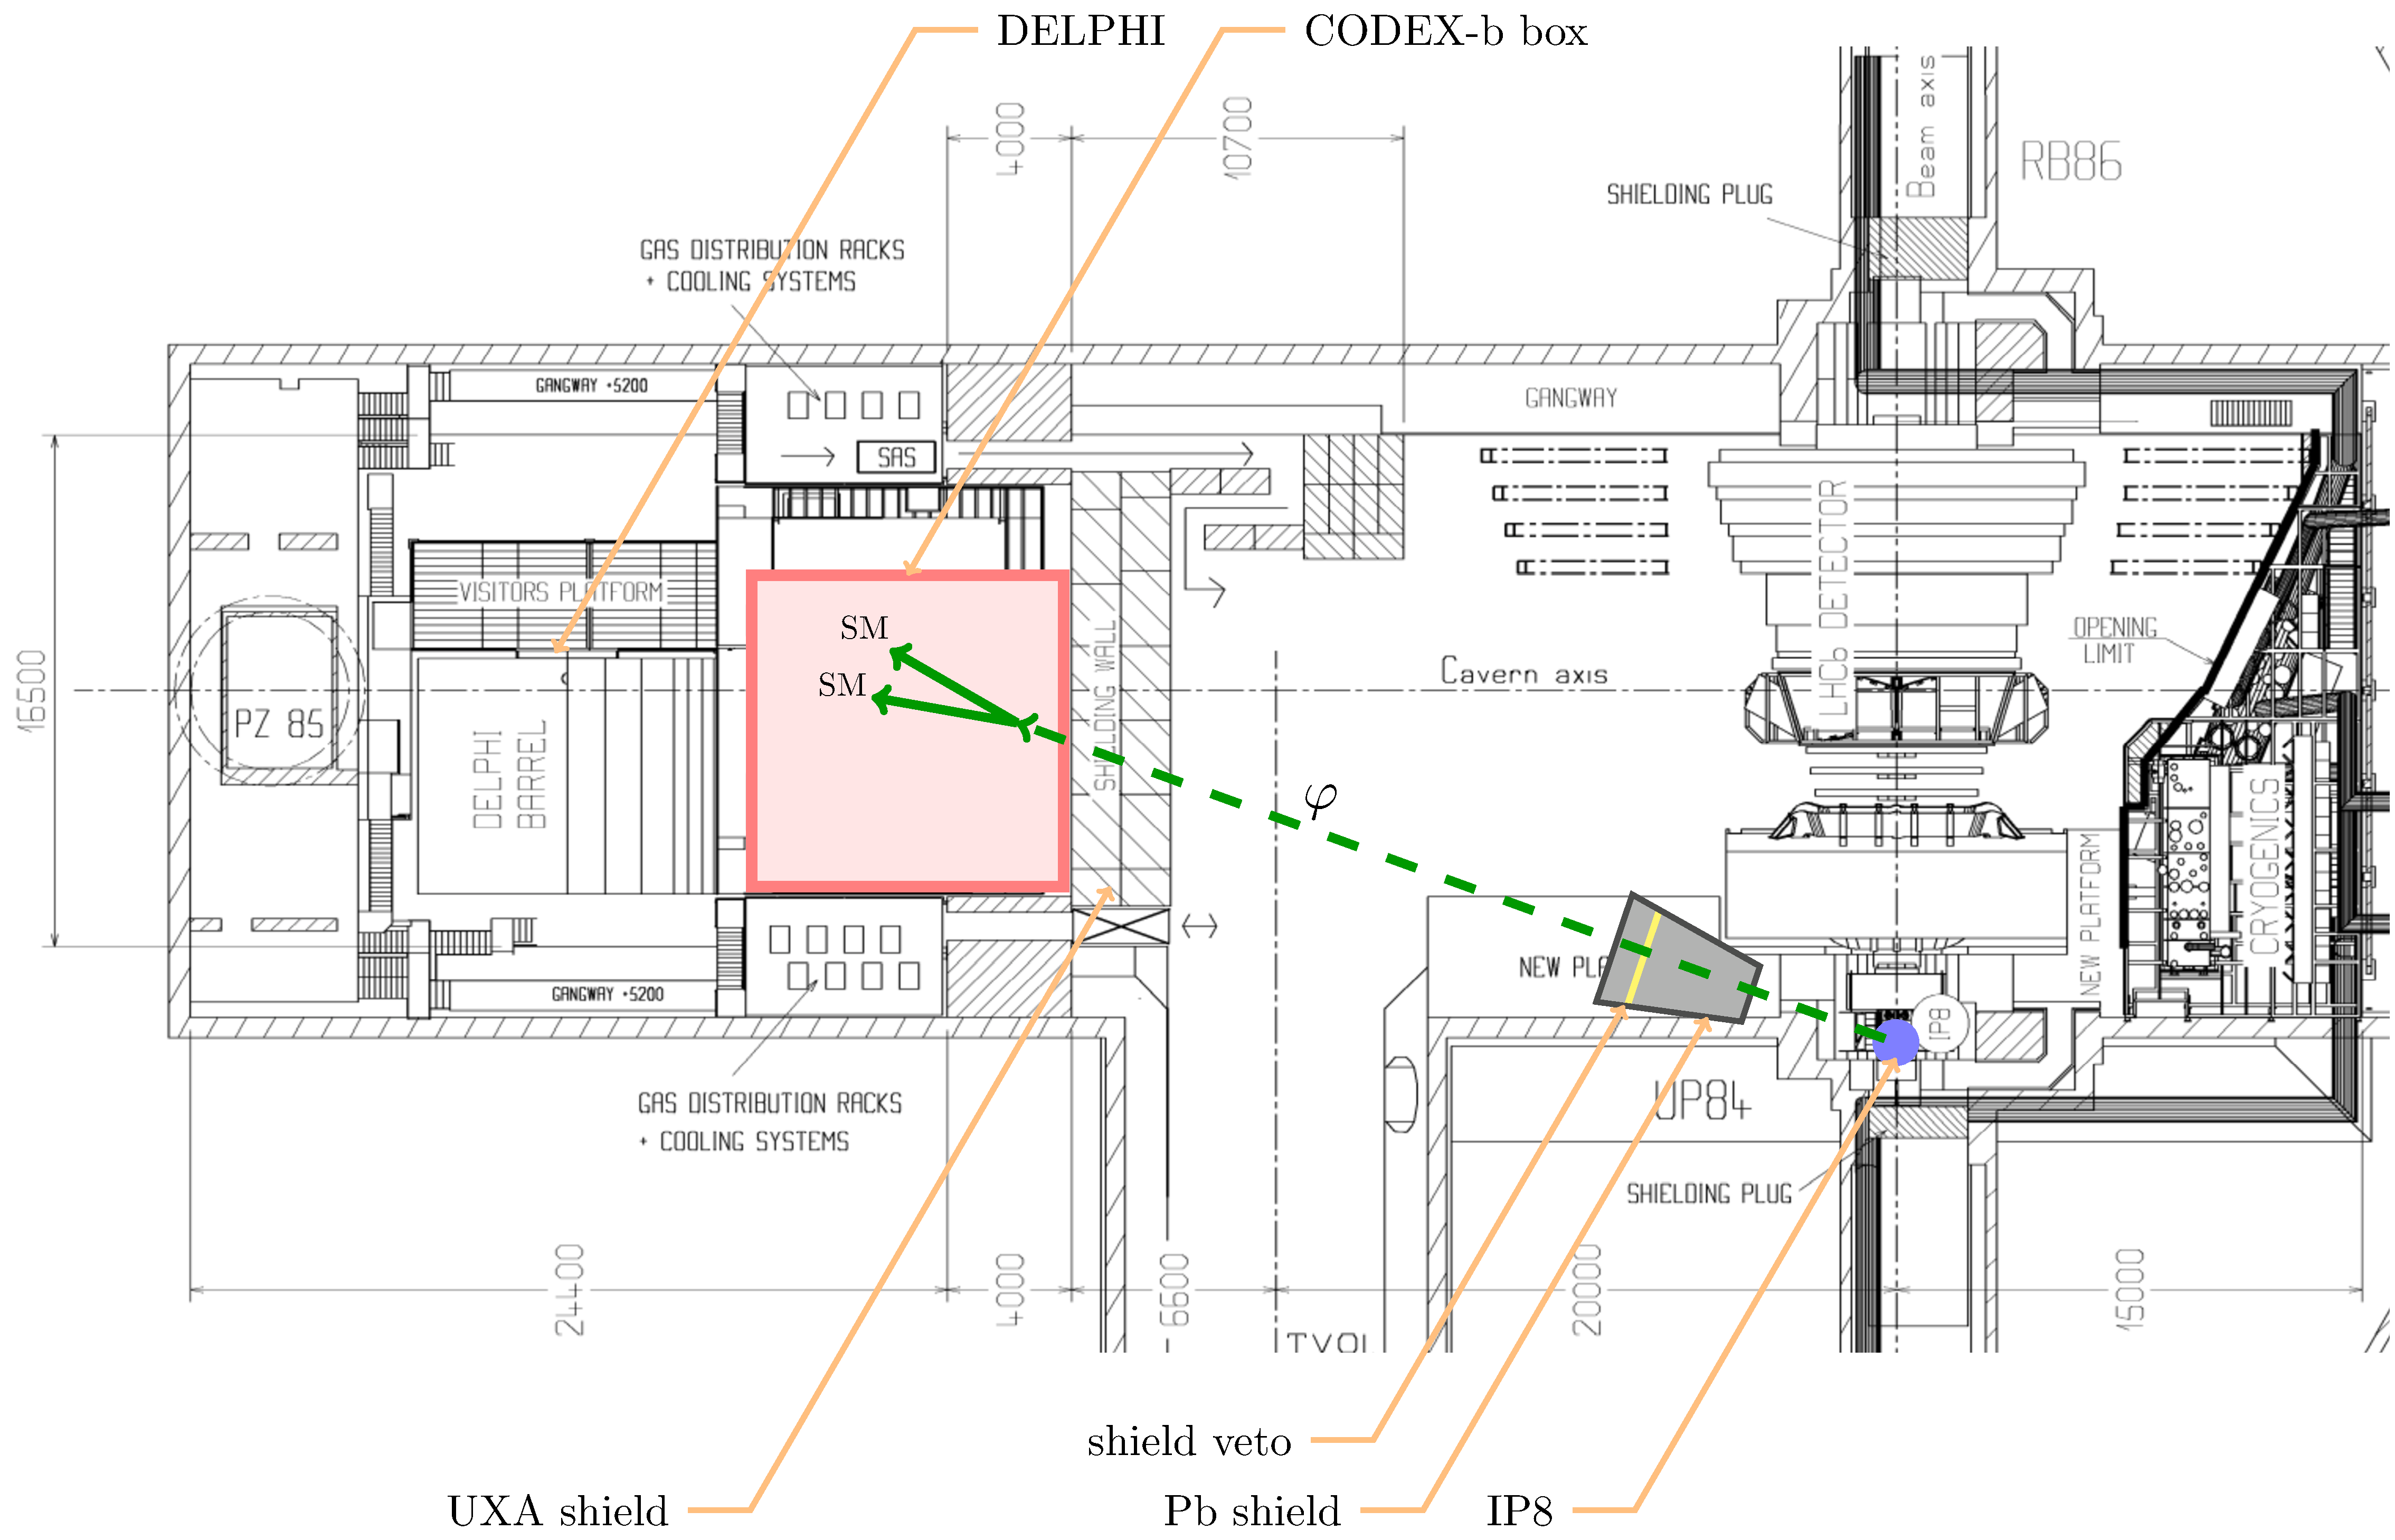
\includegraphics[width = 0.75\linewidth]{plots/LHCbCavern}
	\caption{Layout of the LHCb experimental cavern UX85 at point 8 of the LHC~\cite{cavern}, overlaid with the proposed CODEX-b location.} 
	\label{fig:LHCbCav}
\end{figure}

For the purposes of this white paper, we quantify the reach of CODEX-b for two benchmark models:
% (i) A light scalar which mixes with the Higgs and a (ii) a dark photon which is primarily produced through an exotic Higgs decay.
First we consider light scalar field, $\X$, that mixes with the SM Higgs boson. If $m_\X\lesssim$ 5 GeV, the production mode is primarily through 
inclusive $b \rightarrow s \X$ decays~\cite{Willey:1982dk,Chivukula:1988lo,Grinstein:1988yu}. The LLP $\X$ subsequently decays back to SM fermions through the same Higgs portal. The reach in terms of $m_\X$ and the mixing angle $s_\theta$ is shown in the left-hand panel of Fig.~\ref{fig:ThVM}. CODEX-b significantly extends the projected reach of LHCb using only VELO-based displaced vertex reconstruction, and covers part of the projected parameter of SHiP~\cite{Lanfranchi:2243034} and MATHUSLA  \cite{Evans:2017lvd}. Studies of the potential LHCb reach to longer lifetimes using downstream tracking are ongoing~\cite{Sierra:2017tw,Aaij:2244312}. The right-hand panel of Fig.~\ref{fig:ThVM} indicates the reach for more general models, where the lifetime and production rate of $\X$ are unrelated.


\begin{figure}[t]\centering
	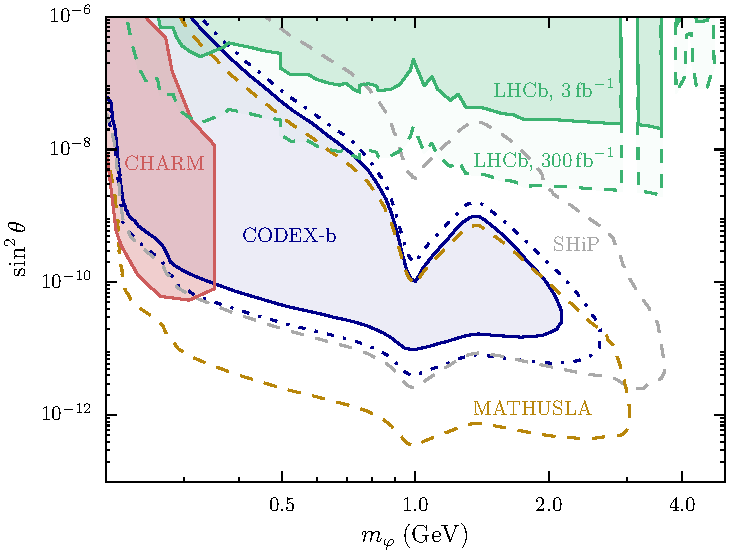
\includegraphics[height =  5cm]{plots/moneyplot_whitepaper.pdf}\hspace{2cm}
	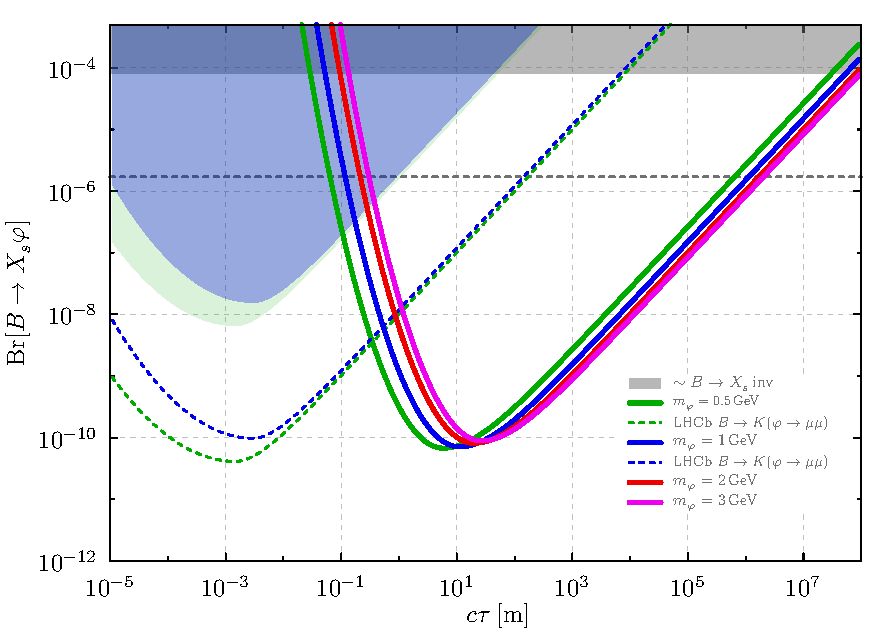
\includegraphics[height = 5cm]{plots/cTauB}
	\caption{\emph{Left:} CODEX-b reach for $B\rightarrow X_s\X$ in the $s^2_\theta$--$m_\X$ plane. Solid (dot-dashed) line assumes $\mathcal{L} = 300\, \text{fb}^{-1}$ ($\mathcal{L} = 1\, \text{ab}^{-1}$).
	\emph{Right:} Inclusive CODEX-b $B \to X_s \X$ reach (solid lines). The shaded regions (dashed lines) indicate current LHCb limits (300$\,$fb$^{-1}$ projection) from $B \to K(\X \to \mu\mu)$, rescaled to the inclusive process and assuming $\text{Br}[\X \to \mu\mu] \simeq 30\%$  and $10\%$ for $m_\X = 0.5$~GeV and $1$\,GeV, respectively. Gray shading and dashed line indicate respectively the approximate current~\cite{PDG:2016} and Belle II projected~\cite{BelleIIreport} limits from $B \to K^{(*)}\nu\bar\nu$ precision measurements.	
	} 
	\label{fig:ThVM}
\end{figure}

For our second benchmark, we consider a dark boson, $\gd$, produced through the exotic Higgs decay $h\rightarrow\gd\gd$. For concreteness we take $\gd$ to be a spin one field which can decay through mixing with the Standard Model photon~\cite{Schabinger:2005ei,Gopalakrishna:2008dv,Curtin:2014cca,Strassler:2008bv}.  In this benchmark, the production and decay are therefore controlled by different portals. The projected reach is shown in Fig.~\ref{fig:HXX}, overlaid with the reach of ATLAS \cite{Coccaro:2016lnz,ATLAS-CONF-2016-042} and MATHUSLA \cite{Chou:2016lxi}. In particular at low $\gamma_d$ masses, CODEX-b complements and significantly extends the reach of ATLAS and CMS.




\begin{figure}[t]\centering
	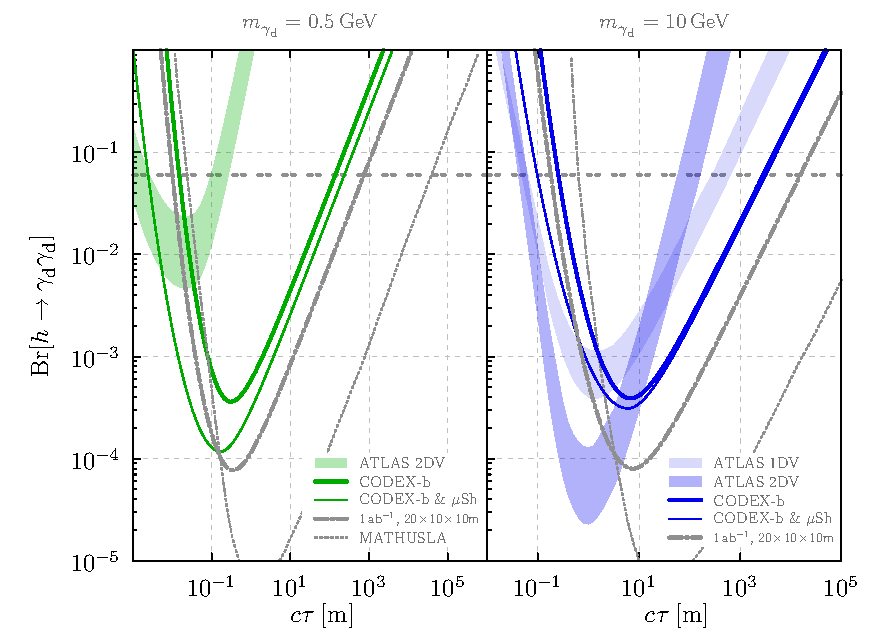
\includegraphics[height =  6cm]{plots/cTau_panel}
	\caption{Higgs decay to dark photon reach with and without the muon shadow (`$\mu$Sh'). The $\gd \to \mu\mu$ branching ratio is taken from $e^+e^-$ data~\cite{Meade:2009rb}. Also included is the optimistic CODEX-b reach with $\mathcal{L} = 1$\,ab$^{-1}$ and a larger volume, assuming DELPHI is removed. }
	\label{fig:HXX}
\end{figure}

\subsection{MoEDAL experiment and future developments}
\label{sec:MoEDAL}

\noindent {\bf Contributors:}~Philippe Mermod, Vasiliki A.\ Mitsou, James L.~Pinfold

\subsubsection{Introduction}\label{sc:intro}

MoEDAL (Monopole and Exotics Detector at the LHC)~\cite{Pinfold:2009oia}\footnote{For general information on the MoEDAL experiment, see: \url{http://moedal.web.cern.ch/}.} is designed to search for manifestations of new physics through highly-ionising (HI) particles in a manner complementary to ATLAS and CMS~\cite{DeRoeck:2011aa}. The main motivation for the MoEDAL experiment is to pursue the quest for magnetic monopoles at LHC energies. Nonetheless the detector is also designed to search for any massive,  long-lived, slow-moving particle~\cite{Fairbairn:2006gg,Burdin:2014xma} with single or multiple electric charges arising in many scenarios of physics beyond the Standard Model~\cite{Acharya:2014nyr}. 

%%%%%%%%%%%%%%%%%%%%%%%%%%%%%%%%%%%%%%%%%%%%%%%%%%%
%%%%%%%%%%%%%%%%%%%%%%%%%%%%%%%%%%%%%%%%%%%%%%%%%%%
\subsubsection{The MoEDAL detector}\label{sc:detector}

The MoEDAL detector~\cite{moedal} is deployed around the intersection region at the LHC Point~8 (IP8) in the LHCb Vertex Locator (VELO) cavern. A schematic view of the MoEDAL experiment is shown in Fig.~\ref{fg:moedal-lhcb}. It is a unique and largely passive detector comprising different detector technologies. 
\begin{figure}[htb]
\begin{minipage}[b]{0.55\textwidth}
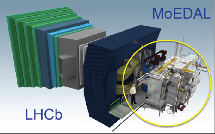
\includegraphics[width=\textwidth]{plots/moedal-detector}
\end{minipage}\hspace{0.05\textwidth}%
\begin{minipage}[b]{0.4\textwidth}
\caption{\label{fg:moedal-lhcb} A three-dimensional schematic view of the MoEDAL detector (in the yellow circle) around the LHCb VELO region at Point~8 of the LHC.}
\end{minipage} 
\end{figure}

%%%%%%%%%%%%%%%%%%%%%%%%%%%%%%%%%%%%%%%%%%%%%%%%%%%
%\subsection{Low-threshold nuclear track detectors}\label{sc:ndt}
\subsection{Nuclear track detectors}\label{sc:ndt}

The main sub-detector system is made of a large array of CR39$^{\tiny{\textregistered}}$,  Makrofol$^{\tiny{\textregistered}}$ and Lexan$^{\tiny{\textregistered}}$ nuclear track detector (NTD) stacks surrounding the intersection area. The passage of a HI particle through the plastic detector is marked by an invisible damage zone along the trajectory. The damage zone is revealed as a cone-shaped etch-pit when the plastic detector is chemically etched. Then the sheets of plastics are scanned looking for aligned etch pits in multiple sheets. The MoEDAL NTDs have a threshold of $Z/\beta\sim5$, where $Z$ is the charge and $\beta=v/c$ the velocity of the incident particle. 

Another type of NTD installed is the Very High Charge Catcher ($Z/\beta\sim50$). It consists of two flexible low-mass stacks of Makrofol$^{\tiny{\textregistered}}$, deployed in the LHCb acceptance between RICH1 and the Trigger Tracker. It is the only NTD (partly) covering the forward region, adding only $\sim0.5\%$ to the LHCb material budget while enhancing considerably the overall geometrical coverage of MoEDAL.

%%%%%%%%%%%%%%%%%%%%%%%%%%%%%%%%%%%%%%%%%%%%%%%%%%%
\subsection{Magnetic trappers}\label{sc:mmt}

A unique feature of the MoEDAL detector is the use of paramagnetic magnetic monopole trappers (MMTs) to capture magnetically-charged HI particles. The high magnetic charge of a monopole ---being at least one Dirac charge $g_{\rm D} = 68.5 e$--- implies a strong magnetic dipole moment, which may result in strong binding of the monopole with the nuclei of the aluminium MMTs. In such a case, the presence of a trapped monopole would de detected through the induction technique by measuring the \emph{persistent current}, defined as the difference between the superconducting magnetometer currents before and after the passage of the MMT bar through the sensing coil~\cite{Joergensen:2012gy,DeRoeck:2012wua}. 

%%%%%%%%%%%%%%%%%%%%%%%%%%%%%%%%%%%%%%%%%%%%%%%%%%%
\subsection{TimePix radiation monitors}\label{sc:timepix}

The only non-passive MoEDAL sub-detector is an array of TimePix pixel devices distributed throughout the MoEDAL cavern, forming a real-time radiation monitoring system of HI beam-related backgrounds. The operation in time-over-threshold mode allows a 3D mapping of the charge spreading in the volume of the silicon sensor, thus differentiating between various particles species from mixed radiation fields and measuring their energy deposition.

%%%%%%%%%%%%%%%%%%%%%%%%%%%%%%%%%%%%%%%%%%%%%%%%%%%
%%%%%%%%%%%%%%%%%%%%%%%%%%%%%%%%%%%%%%%%%%%%%%%%%%%
\subsubsection{MoEDAL physics goals}\label{sc:mm}

The MoEDAL detector is designed to fully exploit the energy-loss mechanisms of magnetically charged particles~\cite{Dirac:1931kp,Dirac:1948um,tHooft:1974kcl,Polyakov:1974ek}  in order to optimise its potential to discover these messengers of new physics. There are various theoretical scenarios in which magnetic charge would be produced  at the LHC~\cite{Acharya:2014nyr}: (light) 't Hooft-Polyakov monopoles~\cite{tHooft:1974kcl,Polyakov:1974ek,Vento:2013jua}, electroweak monopoles~\cite{Cho:1996qd,Bae:2002bm,Cho:2012bq,Cho:2016npz,Ellis:2016glu}, global monopoles~\cite{Barriola:1989hx,Drukier:1981fq,Mazur:1990ak,Mavromatos:2016mnj} and monopolium~\cite{Dirac:1948um,Zeldovich:1978wj,Hill:1982iq,Dubrovich:2002gp}. Magnetic monopoles that carry a non-zero magnetic charge and dyons possessing both magnetic and electric charge are predicted by many theories including grand-unified and superstring theories~\cite{Rajantie:2012xh,Rajantie:2016paj,Kephart:2017esj}. 
 
A possible explanation for the non-observation of monopoles so far is Dirac's proposal~\cite{Dirac:1931kp,Dirac:1948um,Zeldovich:1978wj} that monopoles are not seen freely because they form a bound state called \emph{monopolium}~\cite{Hill:1982iq,Dubrovich:2002gp,Epele:2007ic,Epele:2008un} being confined by strong magnetic forces. Monopolium is a neutral state, difficult to detect directly at a collider detector, although its decay into two photons would give a rather clear signal for ATLAS and CMS~\cite{Epele:2016wps}. Nevertheless the LHC radiation detector systems can be used to detect final-state protons $pp\to pXp$ exiting the LHC beam vacuum chamber at locations determined by their fractional momentum losses~\cite{Kalliokoski:2016fjr}. Such technique would be appealing for detecting monopolia. 

The MoEDAL detector is also designed to search for any massive, long-lived, slow-moving particles~\cite{Fairbairn:2006gg,Burdin:2014xma} with single or multiple electric charges  arising in many scenarios of physics beyond the Standard Model. Supersymmetric long-lived particles, quirks, strangelets, Q-balls, and many others fall into this category~\cite{Acharya:2014nyr}.

%%%%%%%%%%%%%%%%%%%%%%%%%%%%%%%%%%%%%%%%%%%%%%%%%%%%%%%%%%%%%%%%%%%%%%%%%%%%%%%%%%%%%%%%%%%%%%%%%%%%%%
\subsection{Searches for monopoles in MoEDAL}\label{sc:lightsearch}

For the 2015 run at 13~TeV, the MMT consisted of 672~aluminium rods for a total mass of 222~kg that were placed 1.62~m from the IP8 LHC interaction point under the beam pipe on the side opposite to the LHCb detector. The MMT bars were analysed and no magnetic charge  $>0.5g_{\rm D}$ was detected in any of the exposed samples when passed through the ETH Zurich SQUID. Hence cross-section limits are obtained for Drell-Yan (DY) pair production of spin-1/2 and spin-0 monopoles for $1g_{\rm D}\leq|g|\leq 5g_{\rm D}$ at 13~TeV~\cite{Acharya:2016ukt,Acharya:2017cio} improving previous bounds set by MoEDAL at 8~TeV~\cite{MoEDAL:2016jlb}. However, the large monopole-photon coupling invalidates any perturbative treatment of the cross-section calculation and hence any result based on the latter is only indicative. This situation may be resolved if thermal production in heavy-ion collisions ---that does not rely on perturbation theory--- is considered~\cite{Gould:2017zwi}.
\begin{figure}[htb]
\begin{minipage}[b]{0.5\textwidth}
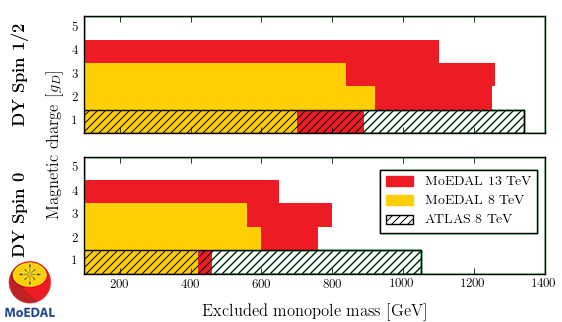
\includegraphics[width=\textwidth]{plots/exclusion3}
\caption{\label{fg:limits} Excluded monopole masses for DY production for spin-$1/2$ (top) and spin-$0$ (bottom) monopoles. The MoEDAL results obtained at 8~TeV~\cite{MoEDAL:2016jlb} and 13~TeV~\cite{Acharya:2016ukt} are superimposed on the ATLAS 8-TeV limits~\cite{Aad:2015kta}.}
\end{minipage}\hspace{0.05\textwidth}%
\begin{minipage}[b]{0.45\textwidth}
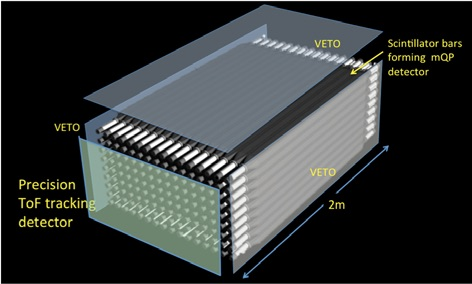
\includegraphics[width=\textwidth]{plots/mapp.jpg}
\caption{A depiction of a MAPP detector subunit. The final detector could contain up to four such units.~\cite{Pinfold:2017dot}.}
\label{fg:mapp}
\end{minipage} 
\end{figure}

Under the assumption of Drell-Yan cross sections, mass limits are derived for $g_{\rm D}\leq|g|\leq4g_{\rm D}$ at the LHC, complementing ATLAS results~\cite{Aad:2012qi,Aad:2015kta}, which placed limits for monopoles with magnetic charge $|g|\leq1.5 g_{\rm D}$, as shown in Fig.~\ref{fg:limits}. The ATLAS bounds are better that the MoEDAL ones for $|g|=1 g_{\rm D}$ due to the higher luminosity delivered in ATLAS and the loss of acceptance in MoEDAL for small magnetic charges. On the other hand, higher charges are difficult to be probed in ATLAS due to the limitations of the level-1 trigger deployed for such searches. Limits on monopole production cross sections set by various colliders are presented in Ref.~\cite{Rajantie:2012xh,Rajantie:2016paj}, while general limits including searches in cosmic radiation are reviewed in Ref.~\cite{Patrizii:2015uea}. 

%%%%%%%%%%%%%%%%%%%%%%%%%%%%%%%%%%%%%%%%%%%%%%%%%%%
%%%%%%%%%%%%%%%%%%%%%%%%%%%%%%%%%%%%%%%%%%%%%%%%%%%
\subsubsection{MoEDAL Apparatus for detecting Penetrating Particles}\label{sc:mapp}

MoEDAL is proposing to deploy the MAPP (MoEDAL Apparatus for detecting Penetrating Particles) in a tunnel shielded by some 30~m to 50~m of rock and concrete from the IP8~\cite{Pinfold:2017dot}. The purpose of the detector is to search for particles with fractional charge as small as one-thousandth the charge of an electron. This detector would also be sensitive to neutral particles from new physics scenarios via their interaction or decay in flight within the volume of the detector. The isolation of the detector means that the huge background from SM processes in the main detectors is largely absent. 

The first apparatus specifically designed to detect mini-charged particles was the SLAC (Stanford Linear Accelerator Centre) `beam dump' type detector, comprising scintillator bars read out by photomultiplier tubes~\cite{Prinz:1998ua}. MoEDAL's new detector, shown in Fig.~\ref{fg:mapp}, and another apparatus proposed for deployment near to the CMS detector~\cite{Haas:2014dda} also designed to search for minicharged particles, both have a design that harks back to the original SLAC detector. In order to reduce backgrounds from natural radiation the photomultiplier tubes and scintillator detectors of the MoEDAL apparatus will be constructed from materials with low natural backgrounds currently utilised in the astroparticle-physics arena. Its calibration system utilises neutral density filters to reduce the received light of high incident muons that manage to penetrate to the sheltered detector from the interaction point, in order to mimic the much lower light levels expected from particles with fractional charges.

%%%%%%%%%%%%%%%%%%%%%%%%%%%%%%%%%%%%%%%%%%%%%%%%%%%
%%%%%%%%%%%%%%%%%%%%%%%%%%%%%%%%%%%%%%%%%%%%%%%%%%%
\subsubsection{Monopoles trapped in beam pipes}\label{sc:pipes}

The possibility of analysing decommissioned parts of the LHC beam-pipe system at the ATLAS, CMS and LHCb/MoEDAL sites with a SQUID to search for trapped magnetic monopoles has been proposed~\cite{beampipe-proposal}. In this context the MoEDAL experiment may serve as a formal platform for coordinating machining, scanning and analysis work, in collaboration with interested ATLAS, CMS and LHCb members. 

The induction technique has been successfully employed at the LHC with the dedicated MoEDAL trapping detector. Additional searches for trapped monopoles in beam-pipe material would access wide windows of magnetic charges and production cross sections to which other LHC experiments are insensitive. The decommissioned central beryllium beam-pipe sections of ATLAS and CMS, with a $4\pi$ coverage and exposure to the highest rates of 7 and 8~TeV $pp$ collisions, are by far the most attractive samples to be analysed.
